\documentclass[11pt]{article}

\usepackage{alltt,fullpage,graphics,color,epsfig,amsmath, amssymb}
\usepackage{hyperref}
\usepackage{boxedminipage}


\newcommand{\floor}[1]{\lfloor #1 \rfloor}
\newcommand{\ceil}[1]{\lceil #1 \rceil}

\begin{document}
\setlength{\parskip}{.1 in}

\begin{center}
\LARGE
\textbf{CS 598RM: Algorithmic Game Theory, Fall 2020}
\\[0.5ex]
\textbf{HW 2 (due on Wednesday, 28th Oct at 11:59pm CST)}
\end{center}


\noindent{\bf Instructions:}
\begin{enumerate}
\item We will grade this assignment out of a total of 60 points. 
\item Feel free to discuss with fellow students, but write your own answers. If you do discuss a problem with someone then write their
names at the starting of the answer for that problem.
\item Please type your solutions if possible in Latex or doc whatever is suitable. We will upload submission instructions on the course webpage and Piazza.
\item Even if you are not able to solve a problem completely, do submit whatever you have. Partial proofs, high-level ideas, examples,
and so on.
\item Except where otherwise noted, you may refer to lecture slides/notes, and to the references provided. 
You cannot refer to textbooks, handouts, or research papers that have not been listed. If you do use any approved sources, make 
sure you cite them appropriately, and make sure to write in your own words.
\item No late assignments will be accepted.
\item By AGT book we mean the following book: Algorithmic Game Theory (edited) by Nisan, Roughgarden, Tardos and Vazirani. 
Its free online version is available at Prof. Vijay V. Vazirani's webpage.
\end{enumerate}
\medskip
\medskip

\noindent\makebox[\linewidth]{\rule{\textwidth}{0.4pt}}


\begin{enumerate}
%----------------------------------------------------------------------
\item 
\begin{enumerate}
    \item (3 points) The following game has a unique Nash equilibrium. Find
it, and prove that it is unique. (Hint: look for strict dominance.)
\begin{center}
\begin{tabular}{| c | c | c |}
\hline
4, 0 & 1, 1 & 4, 0 \\ \hline
1, 3 & 2, -1 & 3, 5 \\ \hline
0, 1 & 3, 0 & 3, 0 \\
\hline
\end{tabular}
\end{center}

\item (4 points). Construct a single $2 \times 2$ normal-form game that simultaneously
has all four of the following properties:
\begin{enumerate}
\item The game does not have a dominant strategy Nash equilibrium (at least one player does not have a dominant strategy).
\item The game is solvable by iterated weak dominance (so that one pure strategy per player remains).
\item In addition to the iterated weak dominance solution (which is a Nash
equilibrium), there is a second pure-strategy Nash equilibrium.
\item Both players strictly prefer the second equilibrium to the first.
(Hints: the second pure-strategy equilibrium should not be strict; the pure strategy equilibria should be in opposite corners of the matrix.) If you cannot get all four properties, construct an example with as many of the properties as you can.
\end{enumerate}

\item (3 points). Consider the following game:
\begin{center}
\begin{tabular}{| c | c |}
\hline
2, 5 & 1, 5 \\ \hline
7, 1 & 0, 0 \\
\hline
\end{tabular}
\end{center}
Find a correlated equilibrium that places positive probability on all entries of the matrix, except the lower-right hand entry. Try to maximize the probability in the upper-left hand entry.
\end{enumerate}

\item Consider a symmetric $2$ person game between Alice and Bob, with the same strategy set $S$ for both players. Let $A(i, j)$ and $B(i,j)$ denote the payoff of Alice and Bob respectively, when Alice plays $i$ and Bob plays $j$. We say that the game is symmetric if we have that $A(i,j) = B(j,i)$ for all $i,j \in S$, {\em i.e.,} $B=A^T$.

\begin{enumerate}
    \item (2 points) Can a symmetric game have a pure Nash equilibria? (even if all values $A(i,j)$ are different?)
    \item (2 points) Do all symmetric games have pure Nash equilibria?
    \item (6 points) J. Nash showed that every symmetric game has a symmetric equilibrium, i.e., a probability distribution $x\in \Delta(S)$ such that $(x,x)$ is an Nash equilibrium. Using this fact derive a quadratic program to compute a symmetric equilibrium of game $(A,A^T)$. \\
\end{enumerate}

\item The $1$-dimensional Sperner's problem is defined on a 1-dimensional grid from $[0, 2^n-1]$, with each integer being a grid
point. There are two colors, red and blue, represented by $0$ and $1$ respectively. 
There is a Boolean circuit named {\em Color,} which outputs the color ($0$/$1$ bit) of a grid point given its bit representation, such that,
Color($0$) = red, Color($2^n-1$) = blue, and the remaining grid points get any color.

\begin{enumerate}
    \item (4 points) Show that there exists an integer $0\le k \le 2^n-1$ such that Color($k$)=red and Color($k+1$)=blue. Furthermore, we can compute it in $O(n)$ calls to the Boolean circuit ``Color''.
    \item (6 points) Show that checking if there are more than one such $k$s is NP-complete (hint: reduce from 3-SAT).
\end{enumerate}


\item (10 points) In the town of Gamica, there is exactly one police patrol, two police stations ($s$ and $t$), and one robber. The robber plans to target a house on one of the streets at night, say on street $i\in [n]$. If street $i$ is patrolled by the police then they get $r_i$ reward while the robber gets $\zeta_i$ cost, otherwise police's cost is $c_i$ and the robber's reward is $\rho_i$. 

Every night, the police can patrol exactly one route from station $s$ to station $t$. \textcolor{red}{At night all the streets are one way, and the street network forms a DAG}. Design a polynomial time algorithm to compute Stackelberg strategy of the police. \\

{\em (Hint: What is the corresponding DBR problem? Can that be solved in polynomial time?)}

\item Consider the extensive-form game shown in the figure.

\begin{figure}[!ht]
\centering
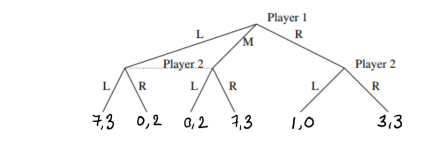
\includegraphics[width=0.5\textwidth]{hw2-Figure.png}
\caption{An extensive-form game with imperfect information.}
\end{figure}

\begin{enumerate}
    \item (3 points). Give the normal-form representation of this game.
    \item (3 points). Give a Nash equilibrium where player $1$ sometimes plays left. (Remember that you must specify each player’s strategy at {\em every} information set.)
    \item (4 points). Characterize the subgame perfect equilibria of the game. (Remember that you must specify each player’s strategy at {\em every} information set.)
\end{enumerate}

\item (10 points) Consider an atomic selfish routing game in which all players have the same source vertex and sink vertex (and each controls one unit of flow). Assume that edge cost functions are non-decreasing, but do not assume that they are affine. Prove that a pure-strategy Nash equilibrium can be computed in polynomial time. Be sure to discuss the issue of fractional vs. integral flows, and explain how (or if) you use the hypothesis that edge cost functions are non-decreasing.
\medskip

[Hint: Recall the Rosenthal's potential function. You can assume without proof that the minimum-cost flow can be solved in polynomial time. If you haven't seen the min-cost flow problem before, you can read about it in any book on ``combinatorial optimization''.]

\end{enumerate}


\end{document}

